\newpage
\subsubsection{三次元計測(飯島・黒崎)}
三次元計測システムの処理は大きく分けて以下のような3つの工程に分けられる.
\begin{itemize}
	\item[工程A.] カメラキャリブレーション(処理1,処理2)
	\item[工程B.] 測定対象の撮影(処理3)
	\item[工程C.] 画像処理(処理4$\sim$処理8)
\end{itemize}

三次元計測システムのフローチャートを図\ref{fig3-9-2-2-1}に示す.図\ref{fig3-9-2-2-1}中では,黒色の四角マークが「処理」,青色のデータマークが「各処理によって作成されたデータ」を示している.

三次元計測システムは処理1から処理9までの計9処理で行われる.(工程A)カメラのキャリブレーションが処理1,処理2,(工程B)撮影対象の撮影が処理3,(工程C)画像処理が処理4から処理8に対応している.

\vspace{2ex}
工程Aで作成されるデータ(レンズパラメータ,ステレオパラメータ)はカメラの設計値に依存する固有値である.すなわち,2度目以降の測定では,工程Aは省略でき,工程B(処理3. 計測対象撮影)以降のみを行えばよい.ただし,カメラ位置や鏡筒長さを変更してしまった場合はもう一度,工程Aからやり直す必要がある.

\subsubsection*{三次元計測時に使用するアプリケーション}
\begin{itemize}
	\item[(1)] GaZooCapture:図\ref{fig3-9-2-2-1}の「処理1. チェッカーボード撮影」および「処理3. 計測対象撮影」で使用する.
	ステレオカメラは2台同時に撮影する必要があるので,PCを2台用意し,各PCにこのアプリケーションを入れておく必要がある.
	
	\item[(2)] MATLAB:図\ref{fig3-9-2-2-1}の「処理2. ステレオキャリブレーション」および「処理4. レンズ歪み補正」以降の処理で使用.
\end{itemize}

\textbf{GaZooCapture使用時に関するコメント}
\begin{itemize}
	\item デバイスが認識されないトラブル多々あった.それは接続不良かカメラ自身の故障が原因.接続不良は接続部分がちゃんと接続されているか確認したり,一度外してもう一度繋げば解決する.カメラ自身の故障はケーブルに張力がかかることが原因.撮影試験の時は,カプトンテープでカメラ本体とケーブルを軽く固定し,ケーブルに張力がかからないように気を付ける.
	
	\item 撮影前にはフォーマット(画像サイズ)と画像の保存形式が間違っていないか確認した方がいい.何度か設定をし忘れ,撮影試験をやり直した.
	
	\item クロスラインを表示することができるので必要に応じて適宜使う.クロスラインを使用することで,カメラの取り付けの際に,2台のカメラの光軸がずれていないかを確かめることができる.
\end{itemize}

\begin{figure}[H]
	\centering
	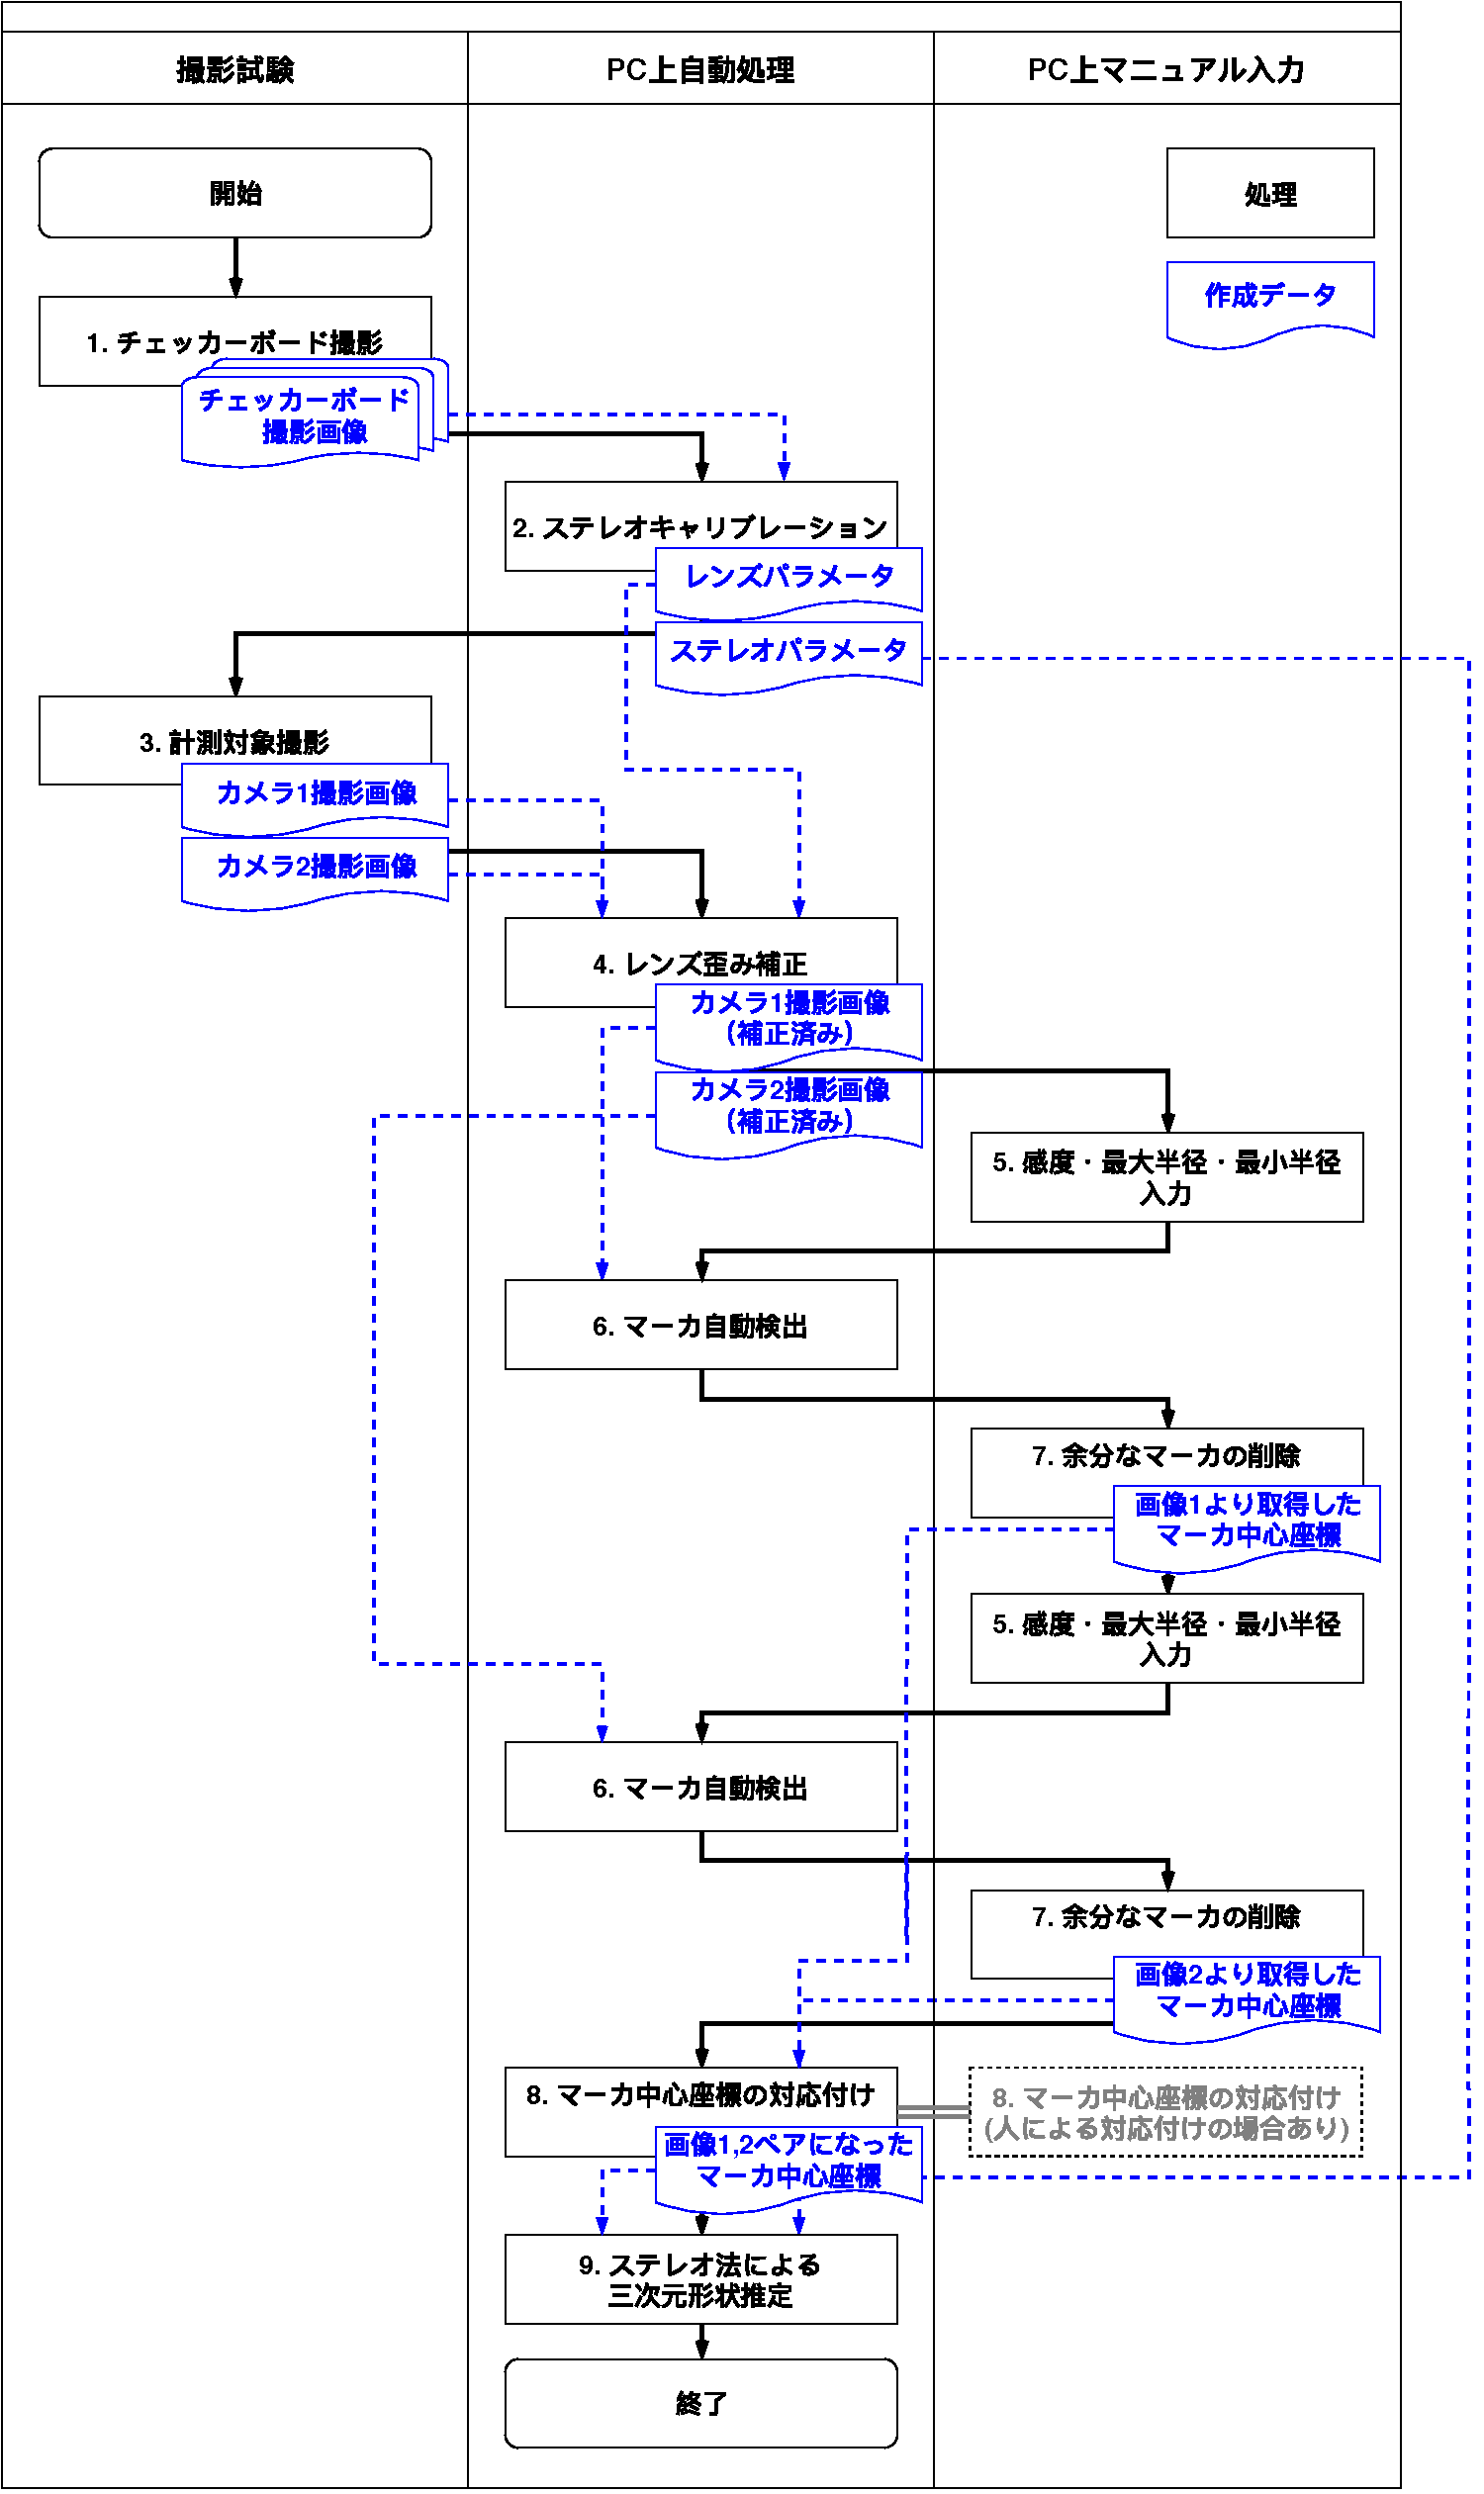
\includegraphics[width=123mm]{03/fig/3-9-2-2-1.pdf}
	\caption{3次元計測システムフローチャート}
	\label{fig3-9-2-2-1}
\end{figure}

\newpage
以下では各処理の詳細について述べる.

\subsubsection*{1. チェッカーボード撮影}
FMカメラのキャリブレーションは,モニターに13マス×19マスのチェッカーボードを映し出し,様々な角度から撮影.チェッカーボードの画像データは,\url{https://helpx.adobe.com/photoshop/digital-negative.html#resources}からAdobe Lens Profile Creatorをダウンロードし,「\yen Adobe\_lensprofile\_creator\_1\_0\_4\_win\yen  lensprofile\_creator\_p4\_win\_072312\yen Adobe Lens Profile Creator 1.0.4\yen calibration charts」というフォルダに入っているデータを使用.撮影枚数は10枚以上あれば何とかなるが,普段は15$\sim$20アングルぐらい,最終キャリブレーションは80アングル撮影した.

\vspace{2ex}
\textbf{コメント}
\begin{itemize}
	\item モニターは解像度の問題があるので,モニターではなく紙に印刷したチェッカーボードを撮影すべきだったかもしれない.紙を使用する場合は,紙がたるまないように注意.モニターと紙のどちらが正解かは分からない.
	\item 13マス×19マスの100\%表示は周りに余白ができていて,スペースがもったいないので,余白が無いようにマス目の多いチェッカーボードを100\%以上で表示させてもいいかもしれない.
	\item 撮影時,カメラ平面に対して チェッカーボードが45 度を超えないように注意.45度を超えた画像が含まれると,キャリブレーション結果が悪くなるらしい.撮影時の注意点は,\url{https://jp.mathworks.com/help/vision/ug/stereo-camera-calibrator-app.html}の「キャリブレーションの改善」に載っている.
\end{itemize}

\subsubsection*{2. ステレオキャリブレーション}
MATLABアプリケーション「ステレオカメラキャリブレーター」を使用.オプションは「半径方向歪み:3つの係数」「計算:せん断・円周方向歪み」を選択.各設定の詳細は,\url{https://jp.mathworks.com/help/vision/ug/stereo-camera-calibrator-app.html}の「キャリブレーションの改善」を参考に.

\subsubsection*{3. 計測対象撮影}
地上暗室実験では,室内のライトを消し暗室で撮影.アルミフレームむき出しだとLEDの明かりによって反射してしまうので,黒い布で隠して撮影を行った.

\subsubsection*{4. レンズ歪み補正}
MATLAB関数「undistortImage」に,「2. ステレオキャリブレーション」で作成されたレンズパラメータと画像データを入力し,画像の歪み補正を行う.

\newpage
\vspace{2ex}
\textbf{コメント}
\begin{itemize}
	\item MATLABではなく,「Adobe Lens Profile Creator」および「Adobe Photoshop」を使用する方法もあったが,Adobe Lens Profile Creatorの設定がよく分からず,誤差が大きくなってしまうことからMATLABのみを使用していた.ただ,まだ完璧に歪みを補正できている訳ではなさそうなので,専門家に確認した方がいいかもしれない.
\end{itemize}

\subsubsection*{5. 感度・最大半径・最小半径を入力}
処理6「マーカ自動検知」において,MATLAB関数「imfindcircles」を使用する場合は事前に,感度,最大半径,最小半径を入力する必要がある.

\vspace{2ex}
\textbf{コメント}
\begin{itemize}
	\item 感度:0.85としていた.1つのマーカに対して多重検知してしまう場合は,感度の値を小さくする(0.7ぐらい)ことによって,解決することができた.

	\item 最大半径・最小半径:被写体距離によって変わる.画像上においてマーカ直径が何ピクセルかを事前に確認しておき,$±$1$\sim$5ピクセルぐらいに設定していた.
	
	\item 感度,最大半径・最小半径によってマーカの中心座標検知精度が変わりそうな気がするので,三次元形状計測精度に関する研究を行う場合は,この3つの数値を気を付ける必要あり.
\end{itemize}

\subsubsection*{6. マーカ自動検出}
MATLAB関数「imfindcircles」を使用.

\subsubsection*{7. 余分なマーカの削除}
格子状配置マーカ対応付けプログラム,旧ランダム配置マーカ対応付けプログラムの場合は,余分なマーカを削除して,画像1と画像2のマーカ数と配置を揃えなければならない.新マーカランダム配置対応付けプログラムの場合は,マーカ以外の変なところを誤検知している場合は削除する必要があるが,マーカ数と配置を完全に一致させる必要はない.

\subsubsection*{8. マーカ中心の対応付け}
(a)格子状配置マーカ対応付けプログラムと(b)ランダム配置マーカ対応付けプログラムの2種類がある.

\subsubsection*{9. ステレオ法による三次元形状計測}
MATLAB関数「triangulate」を使用.


